\documentclass{beamer}

\usepackage[utf8]{inputenc}
\usepackage[T1]{fontenc}
\usepackage[croatian]{babel}
\usepackage{subfigure}
\usepackage{mathtools}

\setbeamertemplate{footline}[frame number]

\title{Detekcija pješaka u urbanim okruženjima korišenjem značajki temeljenih na teksturi i boji}
\author{Iva Miholić, Gustav Matula, Tomislav Kiš}
\makeindex

\begin{document}
\begin{frame}
\maketitle
\end{frame}

\begin{frame}
\frametitle{Sadržaj prezentacije}
\tableofcontents
\end{frame}

\section{Detekcija pješaka u urbanim okruženjima}
\subsection{Opis zadatka}
\begin{frame}
\frametitle{Detekcija pješaka u urbanim okruženjima}
\begin{itemize}
\item detekcija objekta u okviru područja računalnog vida
\item detektor pješaka na fotografijama iz urbanih okruženja korištenjem značajki temeljenih na teksturi i boji
\end{itemize}
\end{frame}

\subsection{Osnovni pregled postojećih rješenja}
\begin{frame}
\begin{itemize}
\frametitle{Osnovni pregled postojećih rješenja}
\item primjena \emph{VJ} detektora objekata \cite{VJ}
\item detektori temeljeni na histogramu usmjerenih gradijenata \emph{Histogram of Oriented Gradients, HOG} \cite{HOG}
\item HOG uz linearni SVM u kombinaciji sa drugim značajkama temeljenih na svojstvima boje, tekstura, oblika, granica, gradijenata
\item složeniji postupci učenja ne daju znatno bolje rezultate \cite{BenensonOHS14}
\end{itemize}
\end{frame}

\begin{frame}
\frametitle{Metoda skalabilnog kliznog prozora}

\begin{figure}
\center
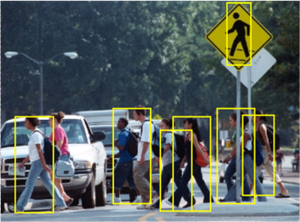
\includegraphics[scale=0.7]{img/crossing.png}
\caption{Fotografija koja je klasificirana detektorom pješaka metodom kliznog prozora. Žuti okviri prikazuju okvire onih prozora koji su klasificirani kao prikaz pješaka.}
\label{primjer_klasifikacije}
\end{figure}
\begin{itemize}
\item ignoriranje konteksta oko okvira koji se promatra 
\end{itemize}
\end{frame}

\section{Baza podataka za treniranje i verifikaciju rješenja }
\begin{frame}
\frametitle{Baza podataka za treniranje i verifikaciju rješenja \\ INRIA \cite{Dollar:2012:PDE:2197081.2197275}}
\begin{figure}
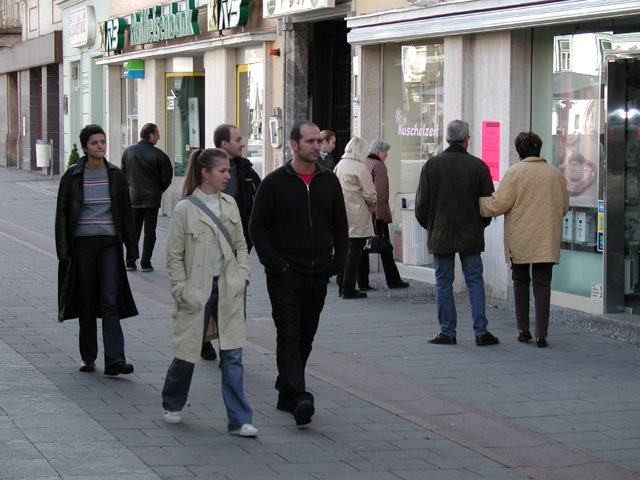
\includegraphics{img/person_139.png}
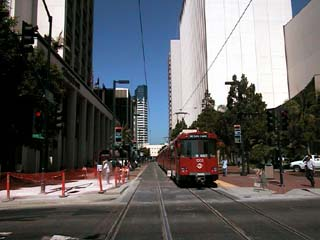
\includegraphics[scale=0.3]{img/neg.png}
\end{figure}
\begin{itemize}
\item{fiksne dimenzije prozora $96 \times 128$}
\end{itemize}
\end{frame}

\section{Pregled značajki temeljenih na teksturi i boji}
\begin{frame}
\frametitle{Pregled značajki temeljenih na teksturi i boji}
\begin{itemize}
\item nadopuna značajkama fokusiranim na bridove (HOG) \cite{HOG}
\item detekcijski prozor podijeljen na preklapajuće blokove u iz kojih se ekstrahiraju značajke
\end{itemize}
\begin{figure}
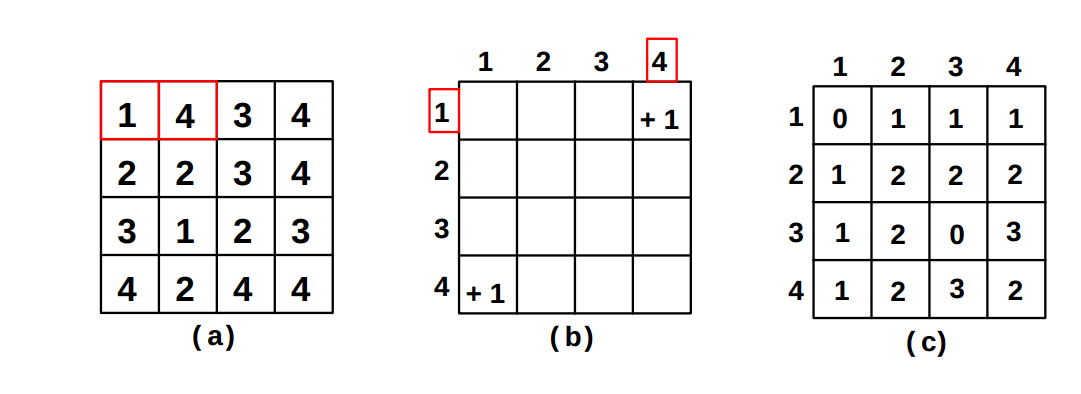
\includegraphics[scale=0.15]{img/matrix.png}
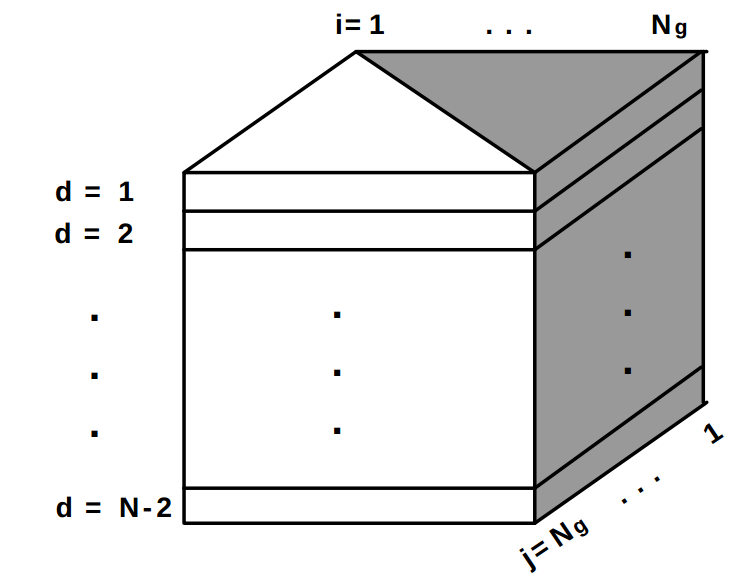
\includegraphics[scale=0.1]{img/cube.png}
\end{figure}
\end{frame}

\subsection{Značajke temeljene na teksturi}
\begin{frame}
\frametitle{Značajke temeljene na teksturi}
\begin{itemize}
\item Haralickov rad \cite{Haralick} -- \emph{co-occurrence} matrica
\item određivanje vjerojatnosti susjedstva svih parova intenziteta
\item primjeri Haralickovih značajki 
\begin{itemize}
\item Varijanca: $$\sum_{i}\sum_{j}(i - \mu)^2p(i, j)$$
\item Korelacija: $$\frac{\sum_{i}\sum_{j}(ij)p(i,j) - \mu_{x}\mu_{y}}{\sigma_{x}\sigma_{y}}$$
\item Entropija: $$-\sum_{i}\sum_{j}p(i, j)\log(p(i, j))$$
\end{itemize}
\end{itemize}
\end{frame}

\subsection{Značajke temeljene na boji}
\begin{frame}
\frametitle{Značajke temeljene na boji}
\begin{itemize}
\item u \cite{Schwartz} jednostavno proširenje HOG histograma
\item promatramo koja boja se najviše mijenja
\item promatramo histogram gradijenata i histogram boja
\end{itemize}
\end{frame}

\subsection{Redukcija dimenzije prostora značajki}
\begin{frame}
\frametitle{Redukcija dimenzije prostora značajki}
\begin{itemize}
\item značajke bliskih blokova su slične -- problem kolinearnosti
\item velika dimenzionalnost problem za klasične metode učenja (SVM)
\item tehnike redukcije dimenzije
\begin{itemize}
\item PCA (\emph{Principal Component Analysis}) 
\item FDA (\emph{Fisher Discriminant Analysis})
\item PLS (\emph{Partial Least Squares})
\end{itemize}
\end{itemize}
\end{frame}

\subsection{PLS - Partial Least Squares}
\begin{frame}
\frametitle{Metoda parcijalnih najmanjih kvadrata - PLS}
\begin{itemize}
\item{dekompozicija $\mathbf{X}$ i $\mathbf{y}$ u nove prostore $\mathbf{T}$ i $\mathbf{U}$ niže dimenzije uz maksimiziranje $cov(\mathbf{T}, \mathbf{U})$:
\begin{equation*}
\mathbf{X} = \mathbf{T} \mathbf{P}^T + \mathbf{E} 
\end{equation*}
\begin{equation*}
\mathbf{y} = \mathbf{U} \mathbf{q}^T + \mathbf{f} 
\end{equation*}
}

\item{Nađi težine $\mathbf{W} = \{\mathbf{w_1}, \mathbf{w_2}, \dots,
\mathbf{w_p} \}$ takve da kovarijance "po stupcima / značajkama" odgovaraju:
\begin{equation*}
[\mathrm{cov}(\mathbf{t_i}, \mathbf{u_i})]^ 2 = \max_{|w_i| = 1} [\mathrm{cov}(\mathbf{X}\mathbf{w_i} ,\mathbf{y})]^ 2
\end{equation*}}
\end{itemize}

\end{frame}

\section{Plan arhitekture sustava računalnog vida}
\begin{frame}
\frametitle{Plan arhitekture sustava računalnog vida}
\begin{enumerate}
\item Treniranje klasifikatora
\begin{figure}[h!]
\center
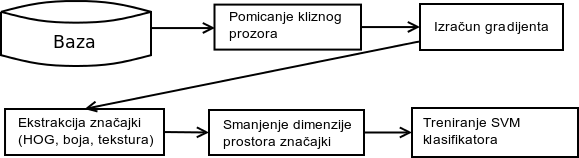
\includegraphics[scale=0.5]{img/treniranje.png}
\caption{Dijagram treniranja SVM klasifikatora}
\label{treniranje}
\end{figure}
\item Testiranje klasifikatora
\item Primjena klasifikatora
\end{enumerate}
\end{frame}

\section{Treniranje klasifikatora i rezultati} 
\begin{frame}
\frametitle{Treniranje klasifikatora}
\begin{itemize}
\item{validacija parametara: \\ vrste jezgre, dimenzije reduciranog prostora; parametara C, $\gamma$ i stupnja polinoma za SVM}
\item{(unakrsna validacija)}
\item{polinomijalna jezgra stupnja $4$\\ reducirani prostor dimenzija $20$}
\item{pogrešno klasificirani negativni primjeri: $29.3\%$}
\item{pogrešno klasificirani pozitivni primjeri: $9.95\%$}
\end{itemize}
\end{frame}

\section{Komentari}
\begin{frame}
\frametitle{Komentari}
\end{frame}

\begin{frame}
\small
\bibliographystyle{ieeetr}
\bibliography{bibliografija}
\end{frame}
\end{document}
